\documentclass[11pt, a4paper]{article}

\usepackage[utf8]{inputenc}
\usepackage[czech]{babel}
\usepackage{graphicx}
\usepackage[a4paper, margin=1in]{geometry}

\title{NUM2 semestrální úkol}
\author{zikmuto2@fjfi.cvut.cz}


\begin{document}
Tomáš Zikmund,  2016/2017, NUM2 semestrální úkol
%\maketitle

\section{Zadání}
Řešte metodou střelby okrajovou úlohu:
\begin{equation}
 -y'' + 16 y = 8, \mbox{kde~} x \in (0,\frac{\pi}{2})
 \label{eq:zadani}
\end{equation}
\[y(0) = \gamma_1 \]
\[y'(\frac{\pi}{2}) = \gamma_2\]

\section{Analytické řešení}
LDR s pravou stranou (\ref{eq:zadani}) má analytické řešení:
\[y(x) = C_1 e^{4x} + C_2 e^{-4x} + \frac{1}{2}\]
Koeficienty \(C_1\) a \(C_2\) z okrajových podmínek určíme vztahy:
\[C_1 = \frac{\frac{\gamma_2}{4} + \left(\gamma_1 - \frac{1}{2}\right) e^{-2\pi}}{e^{2\pi} + e^{-2\pi}}\]
\[C_2 = \gamma_1 - C_1 - \frac{1}{2}\]

%dk:
%\[\gamma_1 = y(0) = C_1 + C_2 + \frac{1}{2} \Rightarrow C_2 = \gamma_1 - C_1 - \frac{1}{2}\]
%\[\gamma_2 = y(\frac{\pi}{2}) = 4 C_1 e^{2\pi} - 4 C_2 e^{-2\pi}
%= 4\left(C_1 e^{2\pi} - \left(\gamma_1 - C_1 - \frac{1}{2}\right) e^{-2\pi}\right)\]
%\[= 4\left(C_1 \left(e^{2\pi} + e^{-2\pi}\right) - \left(\gamma_1 - \frac{1}{2}\right) e^{-2\pi} \right)\]
%\[\Rightarrow C_1 = \frac{\frac{\gamma_2}{4} + \left(\gamma_1 - \frac{1}{2}\right) e^{-2\pi}}{e^{2\pi} + e^{-2\pi}}\]

%Pro případ \(\gamma_1 = 0.1, \gamma_2 = 0.1\) je \(\alpha = y'(0) = -0.4\) a graf analytického řešení je na obrázku \ref{fig:exact}.

\section{Numerické řešení metodou střelby}
LDR s pravou stranou (\ref{eq:zadani}) upravíme na soustavu rovnic:
\[y' = z\]
\[z' = 16 y  - 8\]
\[y(0) = \gamma_1 \]
\[z(\frac{\pi}{2}) = \gamma_2\]

Pro slnění \(z(\frac{\pi}{2}) = \gamma_2\) nalezl progam počáteční podmínku \(\alpha = z(0) = 1.6\).

\subsection{Metoda střelby}
\uv{Zamíříme} pomocí Newtonovy metody vztahem 
\[\alpha^{(k+1)} = \alpha^{(k)} - \frac{F(\alpha^{(k)})}{F'(\alpha^{(k)})}, \]
kde \(F(\alpha) = y'(\frac{\pi}{2};\alpha) - \gamma_2\).

Derivaci \(F'(\alpha) = y_{\alpha}'(\frac{\pi}{2};\alpha)\) určíme řešením úlohy:
\[y_\alpha'' = f_y(x,y,y') y_\alpha + f_{y'}(x,y,y') y_\alpha'\]
\[y_\alpha(0;\alpha)=0, y_\alpha'(\frac{\pi}{2};\alpha) = 1\]
Konkrétně:
\[y_\alpha'(\frac{\pi}{2};\alpha) = \frac{e^{2\pi}+e^{-2\pi}}{2}\]


\begin{figure}
  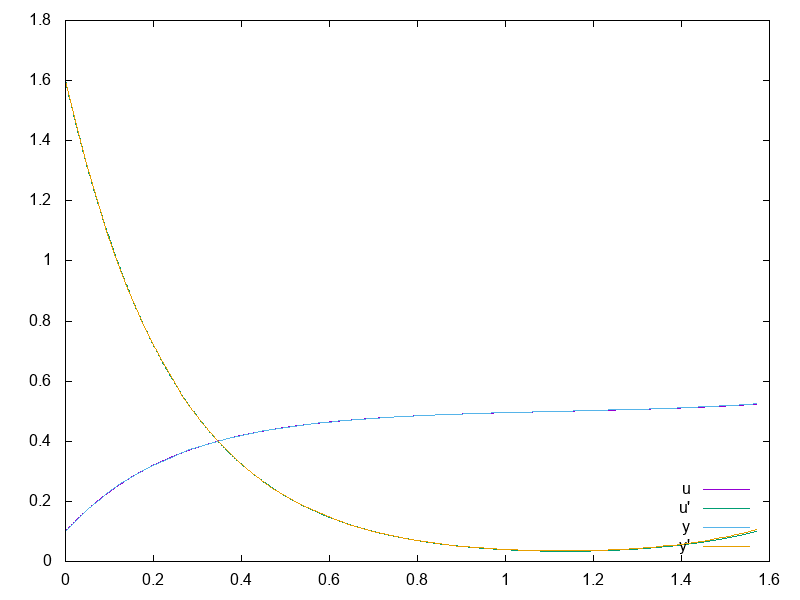
\includegraphics[width=\columnwidth]{img/numeric.png}
  \caption{Graf analytického (y,y') a numerického (u,u') řešení, při \(\gamma_1 = 0.1, \gamma_2 = 0.1\) a \(\alpha = y'(0) = 1.6\). }
  \label{fig:numeric}
\end{figure}

\end{document}
